
\documentclass[template=tabling,81pt,headonall]{azmoon}
\usepackage{xepersian}
\usepackage{amsfonts}
\usepackage{graphicx}
\usepackage{svg}
\svgpath{ {./images/} }
\graphicspath{ {./images/} }
\settextfont{Yas}
\setdigitfont{A Iranian Sans}
\usepackage{fontawesome5}

\printanswers
    \teacher{محمد صالح علی اکبری}
    \teachertitle{دبیر}
    \city{گناباد}
    \schooltitle{متوسطه دوره دوم}
    \school{شهید دکتر چمران}
    \grade{دوازدهم}
    \branch{301}
    \topic{ریاضی}
    \examdate{۱۰/۰۲/۱۴۰۴}
    \answertime{۵۰ دقیقه}
    \begin{document}
	\begin{questions}
		\nointerlineskip%
		\vskip-\baselineskip
		\question[2]{%
نمودار یک تابع با دامنه $(-1,0) \bigcup (0,1) \bigcup (1,2)$ به شکل زیر است. آیا این تابع پیوسته است؟ چرا؟  \\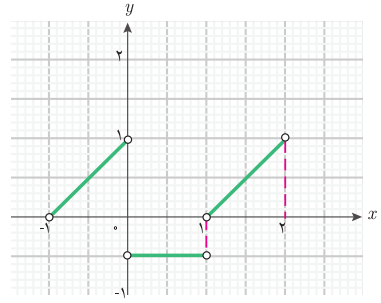
\includegraphics[scale = 0.45]{Screenshot_۲۰۲۵-۰۴-۲۳-۰۶-۰۲-۲۲-۵۹۸_cn.wps.moffice_eng}‌
\\‌
\\}\question[2]{%
نمودار یک تابع به صورت زیر داده شده است. وجود حد این تابع را در نقطه $-2$ ، صفر، $2$ و $3$ بررسی کنید.  \\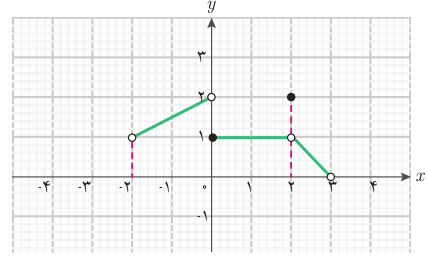
\includegraphics[scale = 0.45]{peyvasteghi_had}‌
\\‌
\\}\question[3]{%
آیا تابع زیر در $x = 2$ حد دارد؟ \\
\begin{equation}
  f(x)=\begin{cases}
    2 - x^2, & \ x <= 2\\
    x - 4, & \ 2 < x
  \end{cases}
\end{equation}
‌
\\‌
\\}\question[3]{%
آیا تابع زیر با دامنه $\mathbb{R}$ در $x = 1$ پیوسته است؟ نمودار این تتابع را رسم کنید. \\
\begin{equation}
  f(x)=\begin{cases}
    1 + x^2, & \ x < 1\\
    0, & \ x = 1\\
    2x, & \ 1 < x
  \end{cases}
\end{equation}
‌
\\‌
\\‌
\\‌
\\‌
\\}\question[4]{%
مشتق تابع های زیر را در نقطه $x = 1$ به دست آورید.
    \begin{LTR}
        \begin{parts}[1]\part{$g(x) = x$}
‌\\‌\\‌\\‌\\\part{$f(x) = x^2$}
\end{parts}
\end{LTR}
        ‌
\\‌
\\‌
\\‌
\\
    }\question[6]{%

مشتق تابع خطی $f(x) = 2x+1$ با دامنه $\mathbb{R}$ را در نقاط $x=1$, $x=3$ و در نقطه دلخواه a حساب کنید.
‌
\\‌
\\‌
\\‌
\\‌
\\‌
\\‌
\\‌
\\}\end{questions}
    \end{document}
    